\documentclass[]{article}
\usepackage{amsmath, amssymb, graphicx}
\graphicspath{{resources/}}


% Title Page
\title{An extension of the formal model for a Library System}
\author{Dominic Rathbone}


\begin{document}
\maketitle
\newpage

\section{Abstract}
The goal of this coursework is to extend and refine the functionality of the existing library system by introducing the concept of time to it in accordance with the requirements given in the coursework document.

\section{Class Invariant}
\subsection{Informal statement}
In order to introduce the concept of time into the library system, a type named "DATE" is created and added to the class invariant. At this level, it is used to define a variable "Today" which is the basis of the system's notion of time. The class invariant has also been extended to add reservations and loans by representing each as a subset of the set resulting from the cartesian product of the sets, title and member. This way, each member of the loan set can be mapped to a "DATE" representing the due date and each member of the reservation subset can be mapped to another "DATE" representing the expiry date . Doing it this way also gives the system more flexibility as this set is not limited to reservations and loans, thus allowing for further extension.
\subsection{Formal statement}
\begin{center}
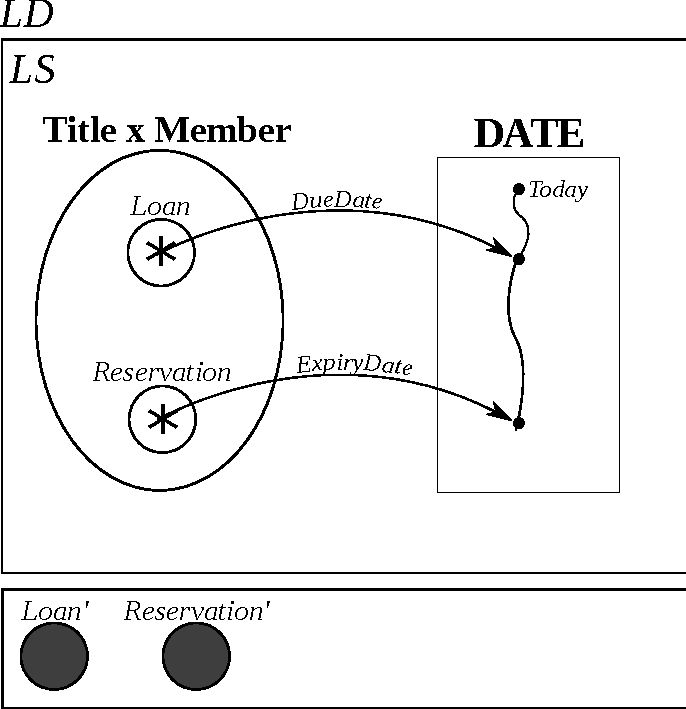
\includegraphics[scale=0.75]{class_invariant.pdf}
\end{center}

\section{Move To Next Day}
\subsection{Informal statement}
Using the "today" variable set up in the class invariant, the next day can be derived. To do so, a new event is created that takes in todays date and increments it by one as allowed by the "DATE" type.
\subsection{Formal statement}
\begin{center}
	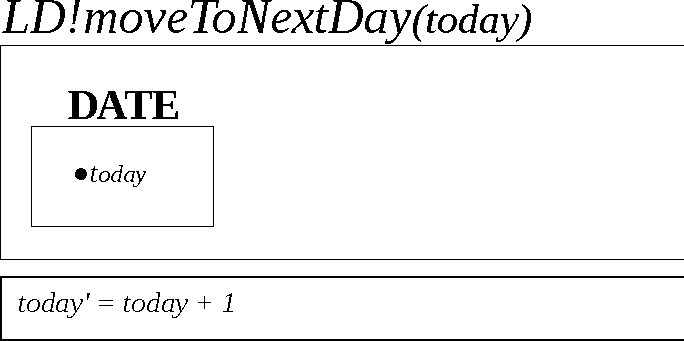
\includegraphics{move_to_next_day.pdf}
\end{center}

\section{Reserve}
\subsection{Informal statement}
The reserve event has to be updated to add a expiry date when a book is reserved. To do this, it has been updated to take new parameters, dur (reservation duration) and today. These are used to calculate the expiry date by adding dur to today's date. A new reservation is then made by pairing title and member then adding it to the reservation set. The expiry date is then linked to this pair by the "ExpiryDate" function.
\subsection{Formal statement}
\begin{center}
	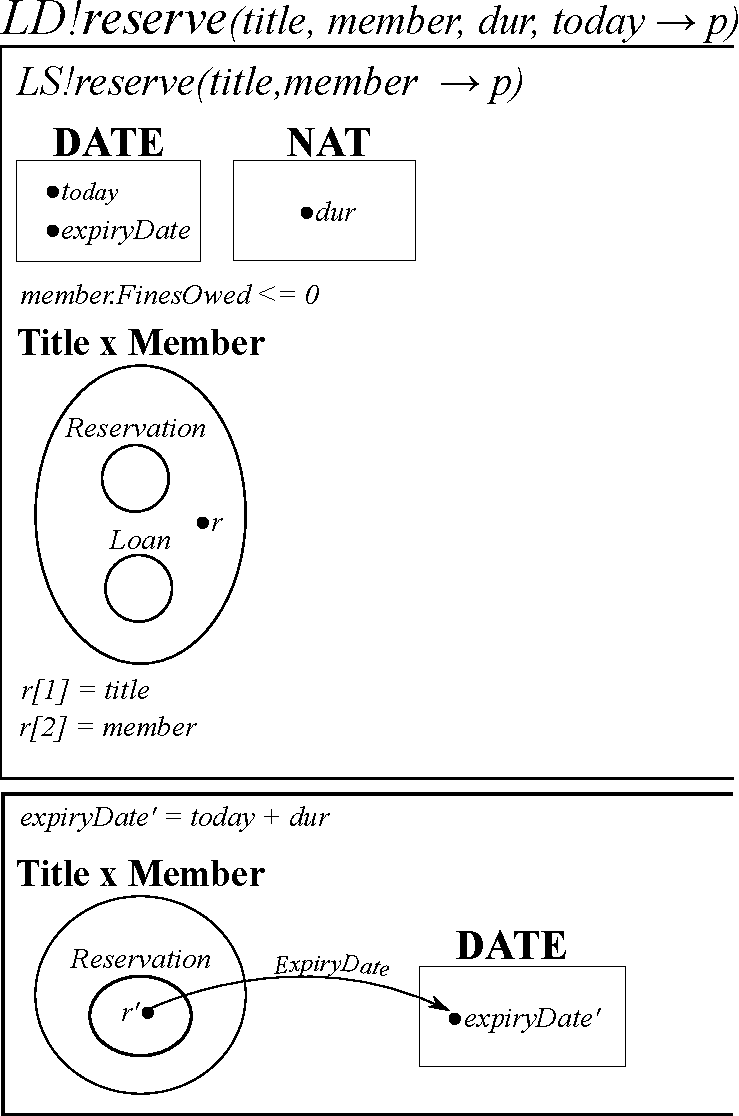
\includegraphics{reserve.pdf}
\end{center}

\section{LoanCopy}
\subsection{Informal statement}
Similar to reserve, the loanCopy event has to be updated to add due dates to new loans taken out. To do this, it is extended to include to new parameters, dur(loan period) and today. From this, the due date is calculated by adding the duration to today. After this, the title and member passed through in the parameter is paired up and linked to the due date by the "DueDate" function.
\subsection{Formal statement}
\begin{center}
	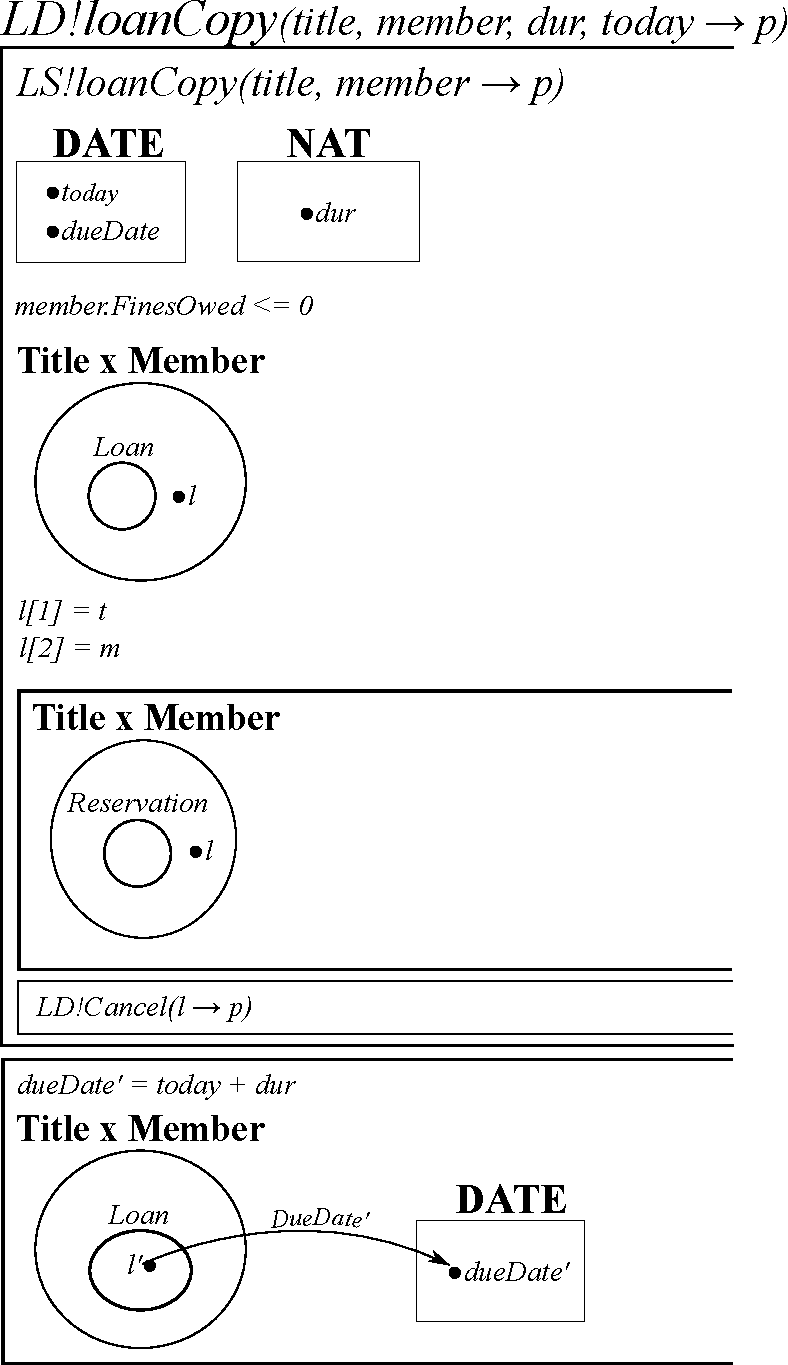
\includegraphics[scale=0.75]{loan_copy.pdf}
\end{center}

\section{Expire}
\subsection{Informal statement}
\subsection{Formal statement}
\begin{center}
	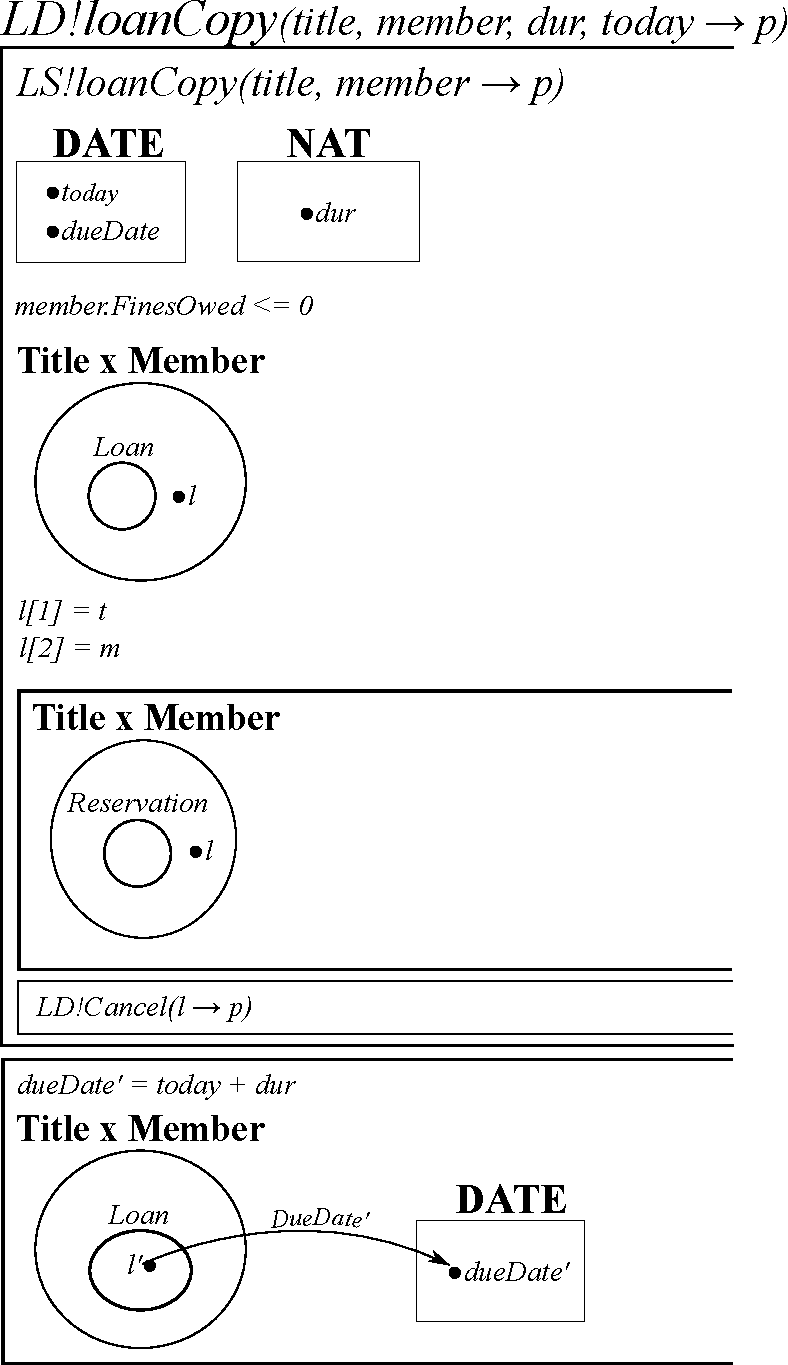
\includegraphics[scale=0.75]{loan_copy.pdf}
\end{center}

\section{Cancel}
\subsection{Informal statement}
\subsection{Formal statement}
\begin{center}
	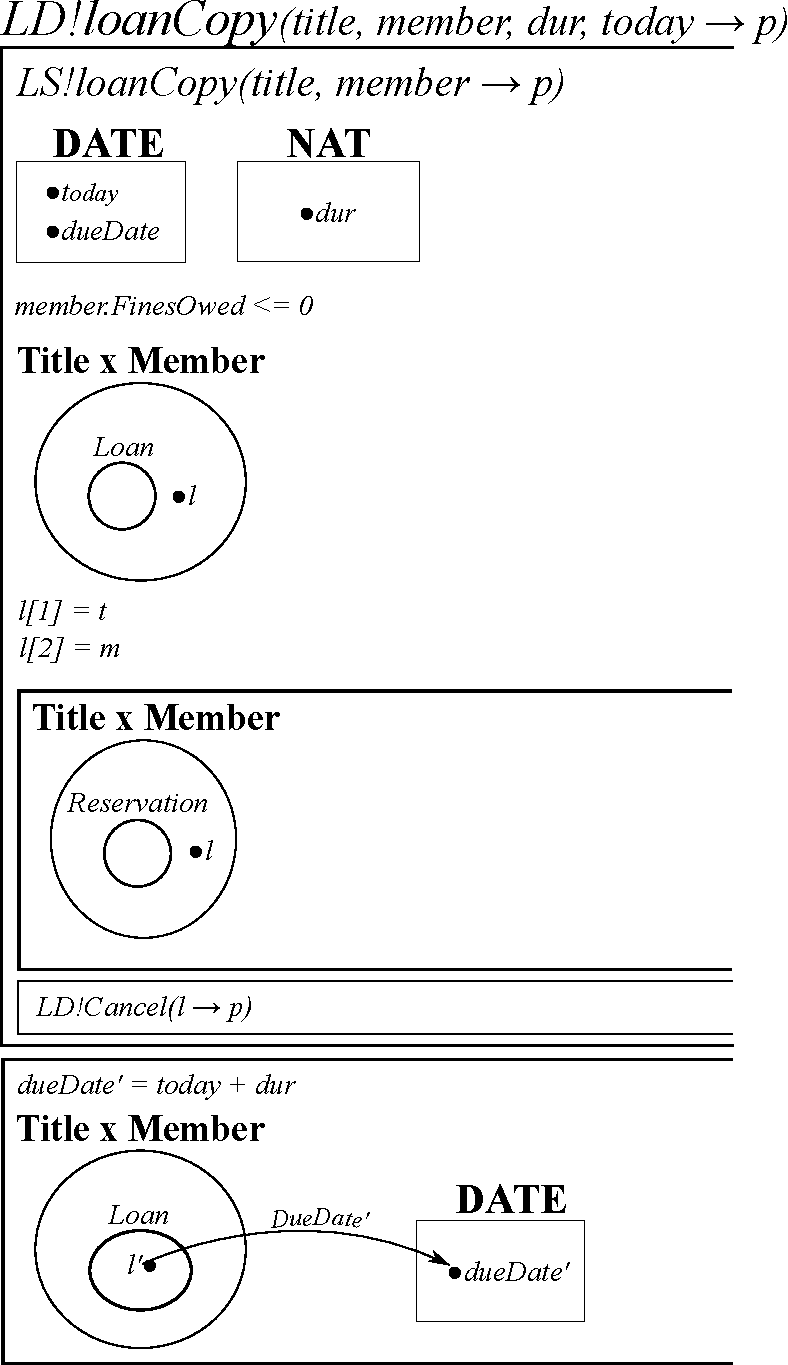
\includegraphics[scale=0.75]{loan_copy.pdf}
\end{center}

\section{ShowDueDate}
\subsection{Informal statement}
\subsection{Formal statement}
\begin{center}
	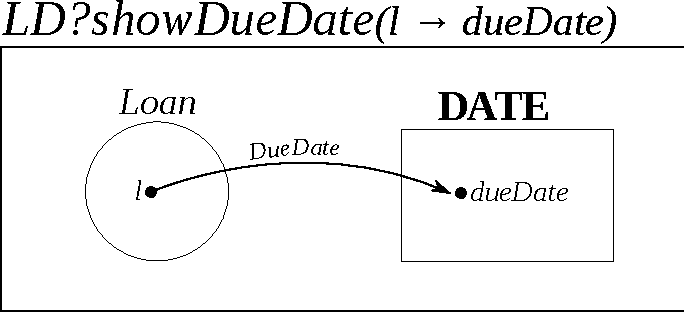
\includegraphics[scale=0.75]{show_due_date.pdf}
\end{center}

\section{ShowExpiryDate}
\subsection{Informal statement}
\subsection{Formal statement}
\begin{center}
	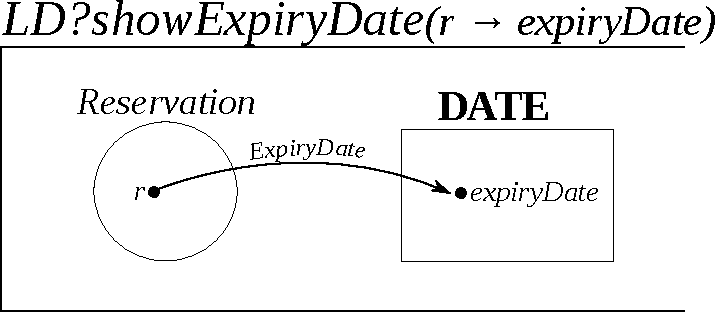
\includegraphics[scale=0.75]{show_expiry_date.pdf}
\end{center}


\end{document}          
